\subsection{CLASP-1 Mutant Model}

In this model, we introduce the CLASP protein to differentiate the wild type root from the CLASP-1 mutant. However, before we do this, it is necessary to confirm that the data from the mutant roots is different from the wild type. We do this by computing the percentage errors from the line of best fit for the wild type data shown in Figure \ref{fig:data-trichoblast}. Plotting these errors gives us a sampling distribution for all three types of roots (Wild Type, BRIN-CLASP, and CLASP-1) which we can compare using statistical methods.  These distributions are shown in Figure \ref{fig:trichoblast-distribution}.

\begin{figure}
    \centering
    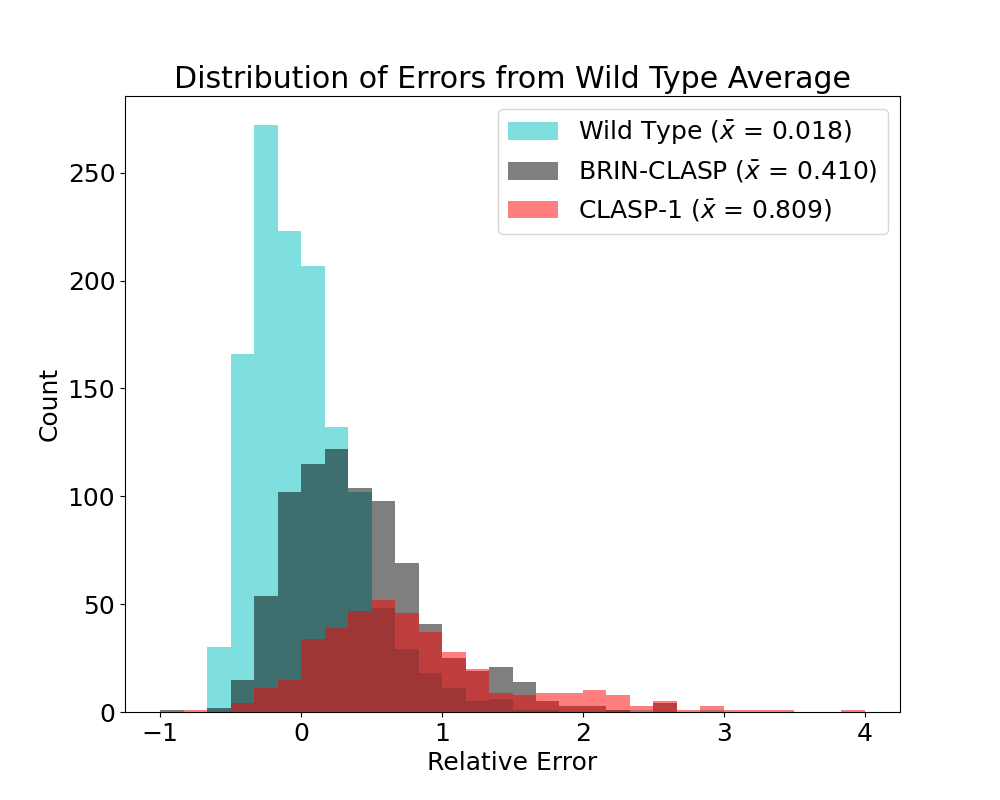
\includegraphics[width=13cm]{img/trichoblast-distribution.png}
    \caption{Distribution of errors from the wild type average presented in Figure \ref{fig:data-trichoblast}. The mean error of the BRIN-CLASP and CLASP-1 mutants are clearly positive, which suggests that the mutants have longer cells compared to the wild type. Both mutants had $p$-values less than $10^{-10}$ when compared to the wild type, which provides further evidence that the mutants are exhibiting different behaviour. }
    \label{fig:trichoblast-distribution}
\end{figure}


\medskip

Now that we have shown quantitatively that the wild type root is different from the CLASP-1 and BRIN-CLASP mutants we are ready to begin defining a system of ODEs for the CLASP-1 mutant model. First, assume that the CLASP protein $C$ is produced at a basal rate $c_{\text{in}}$. As discussed previously, the BES1 transcription factor inhibits CLASP by repressing its promoter (\cite{ruan2018}, so we include a parameter $c_{B}$ that represents this effect. We also include a background degradation rate $c_{\text{out}}$. Since $C$ will not be fitted to experimental data and is thus dimensionless, we will assign an initial condition of $C(0) = 1$. The differential equation defining the CLASP protein is shown in equation \eqref{clasp}.

\begin{equation}
\label{clasp}
\frac{dC}{dt} = c_{\text{in}} - (c_{\text{out}} + c_{B}\text{BES1})
\end{equation}

We also need to integrate the downstream effects of CLASP into our model. Experiments have found that CLASP inhibits growth in a length-dependent manner. Therefore, we add a $g_{C}C / L$ term to the denominator of  equation \eqref{growth} to get the modified version shown in equation \eqref{growth-clasp}. We also omit the $g_{P}$ parameter used in equation \eqref{growth} because this parameter was fit to $0$ in Figure \ref{fig:growth-model-fit}.

\begin{equation}
\label{growth-clasp}
\frac{dL}{dt} = \frac{(g_{B}\text{BES1})L}{1 + (g_{C}C/L)}
\end{equation}

An overview of the entire model incorporating BL, BRI1, BES1, CLASP, and cell growth is presented in Figure \ref{fig:clasp1-model}. The differential equations used in the model were approximated using a forward euler method with time step $0.01\h$. The model accuracy was quantified using the sum of the RMSE from the Wild Type and CLASP-1 data. In CLASP-1 roots we fixed the parameter values $c_{\text{in}} = c_{\text{out}} = c_{B} = 0$ and set the initial condition of the CLASP equation to $0$. Additionally, the CLASP-1 root is given a different initial length parameter $g_{1}$ that may differ from the initial length parameter $g_{0}$ used for the Wild Type.  All other parameters were held constant accross the two root types.

\begin{figure}
    \centering
    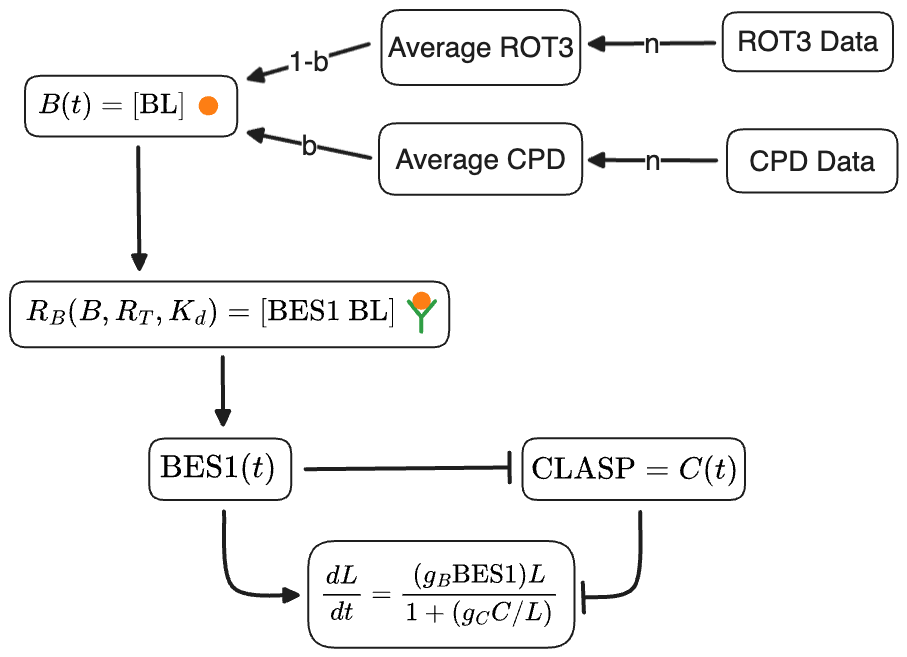
\includegraphics[width=13cm]{img/clasp1-model.png}
    \caption{Our complete model of cell growth in \emph{A. thaliana} which contains the BL concentration $B$, the BRI1 concentration $R_{T}$, the bound receptor concentration $R_{B}$, the level of $\text{BES1}$ signalling, the quantity of CLASP protein $C$, and the length of the cell $L$.}
    \label{fig:clasp1-model}
\end{figure}


